% Created 2020-06-06 Sat 12:14
% Intended LaTeX compiler: pdflatex
\documentclass[11pt]{article}
\usepackage[utf8]{inputenc}
\usepackage[T1]{fontenc}
\usepackage{graphicx}
\usepackage{grffile}
\usepackage{longtable}
\usepackage{wrapfig}
\usepackage{rotating}
\usepackage[normalem]{ulem}
\usepackage{amsmath}
\usepackage{textcomp}
\usepackage{amssymb}
\usepackage{capt-of}
\usepackage{hyperref}
\usepackage{minted}
\author{Dustin Leatherman}
\date{\today}
\title{Optimization Theory: Term Project}
\hypersetup{
 pdfauthor={Dustin Leatherman},
 pdftitle={Optimization Theory: Term Project},
 pdfkeywords={},
 pdfsubject={},
 pdfcreator={Emacs 26.3 (Org mode 9.4)}, 
 pdflang={English}}
\begin{document}

\maketitle
\tableofcontents


\section{Code}
\label{sec:org9206970}
\begin{minted}[]{octave}


%%%%%%%%%%%%%%%%%%%%%%%%%%%%%%%%%%%%%%%%%%%%%%%%%%%%%%%%%%%%%%
%%%
%%%   Make the Data
%%%
%%%%%%%%%%%%%%%%%%%%%%%%%%%%%%%%%%%%%%%%%%%%%%%%%%%%%%%%%%%%

nrow = 60; dimN = 50;  Nsamples = 50; K = 4;
patch = 20 * ones(28, 20);
background = zeros(nrow, dimN);
seed = 13579;
BigPrime = (2^31) - 1;

Xmat = zeros(nrow * dimN, Nsamples);

index = 1;

for corner1 = 4:8
     for corner2 = 4:8
         for jj = 1:nrow
            for kk = 1:dimN
                seed = mod(16807 * seed, BigPrime);
                background(jj, kk) = 4 * (seed / BigPrime);
            end
         end

         picture = background;
         picture([(corner1):(corner1 + 27)],[corner2:corner2 + 19]) = patch;

         Xmat(:,index) = reshape(picture,nrow * dimN,1);
         index = index + 1;
     end
end

for corner1 = 26:30
    for corner2 = 26:30
         for jj = 1:nrow
            for kk = 1:dimN
                seed = mod(16807 * seed, BigPrime);
                background(jj,kk) = 4 * (seed/BigPrime);
            end
         end

        picture = background;
        picture([(corner1):(corner1 + 27)],[corner2:corner2 + 19]) = patch;

        Xmat(:,index) = reshape(picture,nrow * dimN, 1);
        index = index + 1;
    end
end


%%%%%%%%%%%%%%%%%%%%%%%%%%%%%%%%%%%%%%%%%%%%%%%%%%%%%%%%%%%%%%%%%%%%%
%%%
%%% Step 1 of the Algorithm
%%% Find the distance between each pair of data points x_j and x_k
%%% For each data point, find its K nearest neighbours
%%%
%%%%%%%%%%%%%%%%%%%%%%%%%%%%%%%%%%%%%%%%%%%%%%%%%%%%%%%%%%%%%%%%%%%%%

% instantiate dist matrix
dist = zeros(dimN, dimN);

% iterate over pairs of to avoid a nested for-loop
for idx_pair = nchoosek(1:dimN, 2)'

  a = idx_pair(1);
  b = idx_pair(2);

  % calculate distance via euclidean dist
  dist_i = norm(Xmat(:, b) - Xmat(:, a));

  % Populate the coords for the matrix
  % This creates a symmetric matrix of distances
  % the diagonal is always 0 since the distance between an element and itself is 0.
  dist(a , b) = dist_i;
  dist(b , a) = dist_i;
end

% sort each vector in asc order
[dist_srt, idx] = sort(dist);

%%%
%%% each column stores the K nearest neighbours for that data point
%%%

% ignore first value because its always 0 since it refers
% to the column value
knn = idx(2:K + 1, :);

%%%%%%%%%%%%%%%%%%%%%%%%%%%%%%%%%%%%%%%%%%%%%%%%%%%%%%%
%%%
%%% Step 2 of the Algorithm
%%% Solve for the weights for each data point
%%%
%%%%%%%%%%%%%%%%%%%%%%%%%%%%%%%%%%%%%%%%%%%%%%%%%%%%%%%


weights = [];
for col = 1:dimN
  G = zeros(K, K);
  for coords = [nchoosek(1:K, 2); repmat((1:K)', 1, 2)]'

    r = coords(1);
    c = coords(2);

    g = (Xmat(:, col) - Xmat(:, knn(c, col)))' * (Xmat(:, col) - Xmat(:, knn(r, col)));

    G(r, c) = g;
    G(c, r) = g;
  end

  % Apply regularization to weights to guarantee G is non-singular (and thus invertible)
  weight_i = inv(G + 0.001 * eye(K)) * ones(K, 1);

  % adjust the weights so they sum to one.
  % thus satisifying the constraint that weights must sum to one.
  adj_weight_i = weight_i / sum(weight_i);
  weights = [weights adj_weight_i];
end


%%%%%%%%%%%%%%%%%%%%%%%%%%%%%%%%%%%%%%%%%%%%%%%%%%%%%%%%%%%%%%%%%
%%%
%%%  Step 3 of the Algorithm
%%%  Compute the M matrix, call it M_mat
%%%
%%%%%%%%%%%%%%%%%%%%%%%%%%%%%%%%%%%%%%%%%%%%%%%%%%%%%%%%%%%%%%%%%

ident = eye(dimN);

% get pairs of 1-50 and 1-4
% [1 1; 1 2; 1 3; 1 4; ... 50 1; 50 2; 50 3; 50 4]

weights2 = zeros(dimN:dimN);
Klist = [1:K];
% get all combinations.
for coords = nchoosek([1:dimN, 1:K], 2)'
  r = coords(1);
  c = coords(2);

  % only act on combinations where operating on 1:K
  % Would be better to filter this out upfront
  if ismember(r, Klist)
    weights2(c, knn(r, c)) = weights(r, c);
  endif
end

M_mat = (ident - weights2)' * (ident - weights2);
%%%%%%%%%%%%%%%%%%%%%%%%%%%%%%%%%%%%%%%%%%%%%%%%%%%%
%%%%
%%%% compute the eigenvectors of the matrix M_mat
%%%%
%%%%%%%%%%%%%%%%%%%%%%%%%%%%%%%%%%%%%%%%%%%%%%%%%%%%

[V, D] = eig(M_mat);

d = 2;
%%% if the two smallest eigenvalues are both zero,
%%% then use the eigenvectors in the third and fourth column of matrix V.
if diag(D)(1:d) == [0; 0]
  % interested in the (d + 1)st coordinate so 1 is added
  Y_mat = V(:, (d + 2):(d + d + 1));
else
  Y_mat = V(:, 2:(d + 1));
endif

x_axis = Y_mat(:, 1);

y_axis = Y_mat(:, 2);

scatter(x_axis, y_axis)


%%%%%%%%%%%%%%%%%%%%%%%%%%%%%%%%%%%%%%%%%%%%%%%%%%%%%%%%%%%%%%%%%%%%%%
%%%%
%%%%   Verfiy that the calculation of matrix M_mat is done correctly.
%%%%   NOTE: This part is Optional.  Only do this if you wish to discuss your project in job interviews.
%%%%%%%%%%%%%%%%%%%%%%%%%%%%%%%%%%%%%%%%%%%%%%%%%%%%%%%%%%%%%%%%%%%%%%%

% Ugly brute force code just to make sure the answers are right.
cost1 = 0;
for i = 1:dimN
  for j = 1:dimN
    cost1 = cost1 + M_mat(i,j) * (V(:, i)' * V(:, j));
  end
end

cost2 = 0;
for i = 1:dimN
  innercost = 0;
  for j = 1:dimN
    % Use the sparse weights matrix used to calculate M
    innercost = innercost + weights2(i,j) * V(:, j);
  end
  cost2 = cost2 + ((V(:, i) - innercost) .^ 2);
end

% cost2 is a vector so sum the vector to get the cost
cost2 = sum(cost2)

% round to the nth precision. Octave (OpenSource Matlab) only supports round(X), not round(X,N)
round2 = @(x, n=0) round (x * 10^n) * 10^(-n)

% trailing digits differ slightly so rounding for equality check
if round2(cost1, 5) == round2(cost2, 5)
  disp("M_mat calculated correctly!")
else
  disp("M_mat values do not match. Check calculations")
endif

%%% Code for Project output
% plot 3 and 4th eigenvectors
scatter(V(:, 3), V(:, 4))

% plot 4th and 5th eigenvectors
scatter(V(:, 4), V(:, 5))

% output of third eigenvector
>> V(:, 3)
ans =

   0.00000
   0.00000
   0.00000
   0.00000
   0.00000
   0.00000
   0.00000
   0.00000
   0.00000
   0.00000
   0.00000
   0.00000
   0.00000
   0.00000
   0.00000
   0.00000
   0.00000
   0.00000
   0.00000
   0.00000
   0.00000
   0.00000
   0.00000
   0.00000
   0.00000
   0.26858
   0.16758
   0.00685
  -0.15590
  -0.25706
   0.27351
   0.16837
   0.00448
  -0.15856
  -0.26613
   0.27321
   0.17129
   0.00156
  -0.17057
  -0.27476
   0.26851
   0.16263
  -0.00271
  -0.16942
  -0.27619
   0.26031
   0.15909
  -0.00812
  -0.17194
  -0.27460
\end{minted}



\section{Figures}
\label{sec:org16e8489}

\begin{figure}[htbp]
\centering
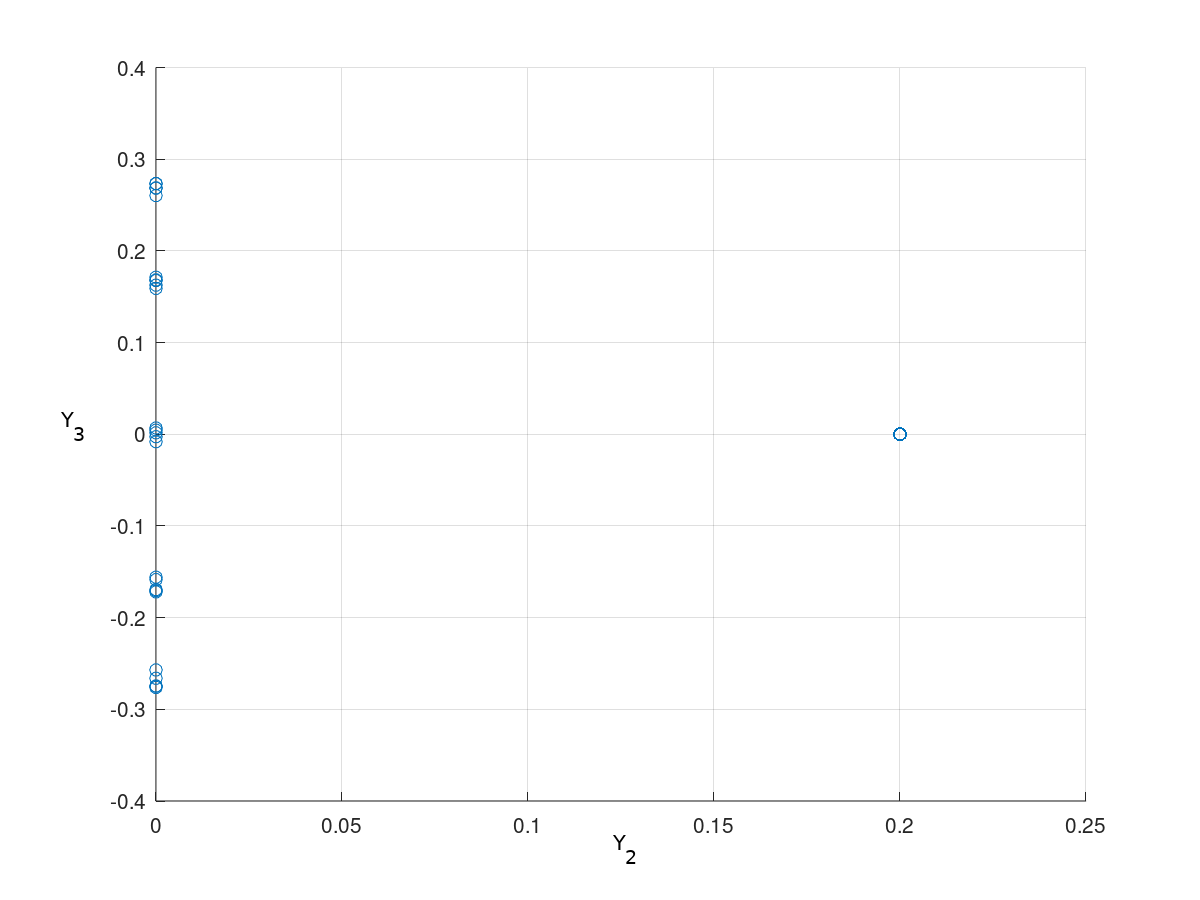
\includegraphics[width=8cm,height=8cm]{./resources/y2y3.png}
\caption{\label{fig:org71ea535}2nd vs 3rd Eigenvectors}
\end{figure}

\begin{figure}[htbp]
\centering
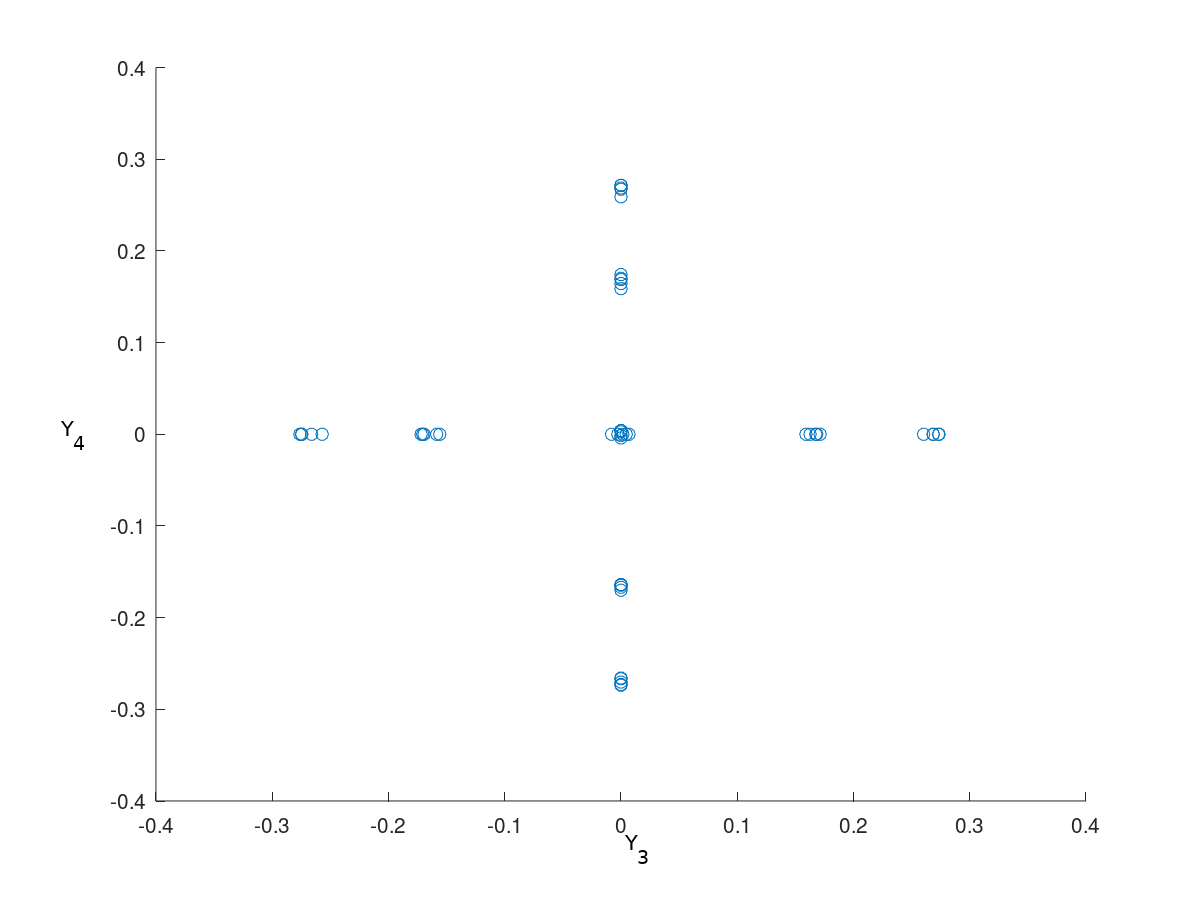
\includegraphics[width=8cm,height=8cm]{./resources/y3y4.png}
\caption{\label{fig:orgeeed81a}3rd vs 4th Eigenvectors}
\end{figure}


\begin{figure}[htbp]
\centering
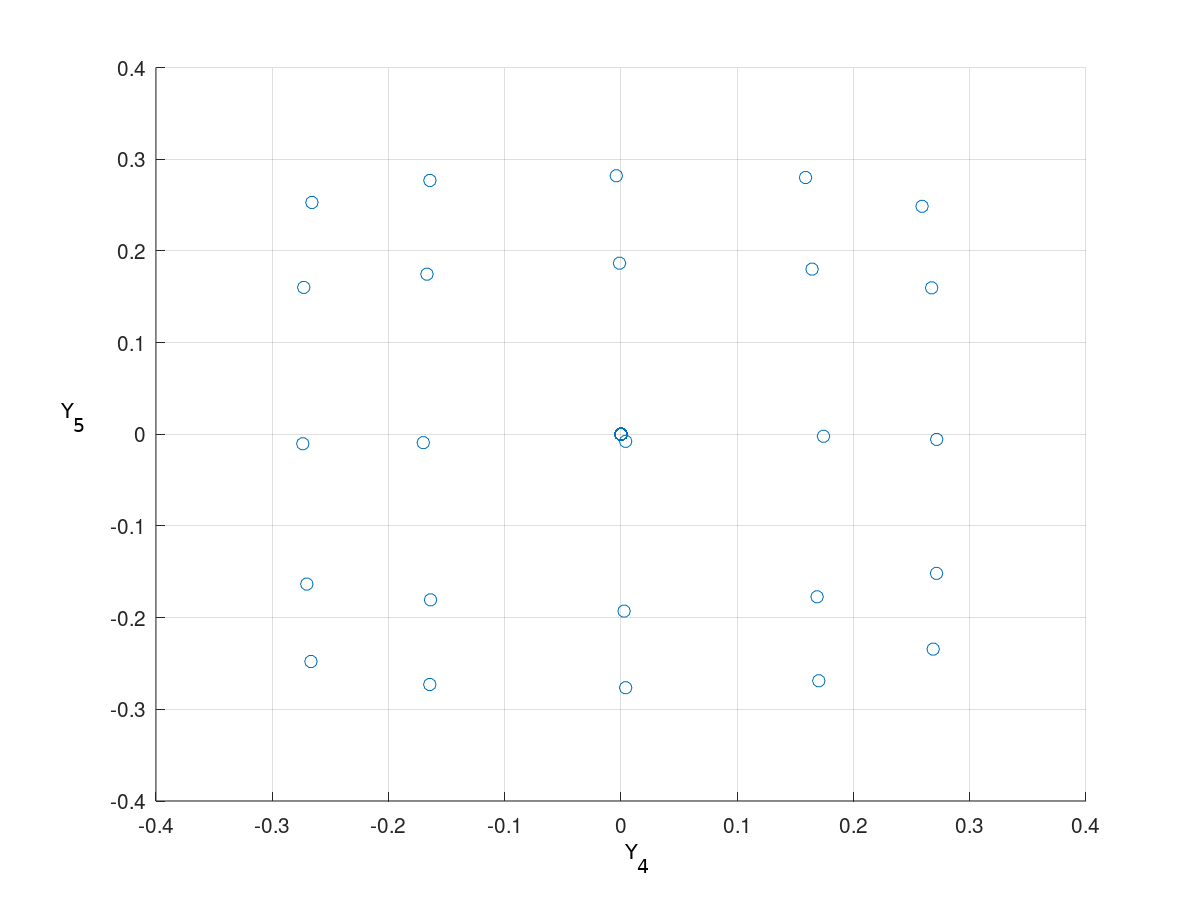
\includegraphics[width=8cm,height=8cm]{./resources/y4y5.png}
\caption{\label{fig:org499b444}4th vs 5th Eigenvectors}
\end{figure}
\end{document}
